
\documentclass[a4paper,12pt]{article}
\usepackage{times}
\usepackage[francais]{babel}
\usepackage[utf8x]{inputenc}
\usepackage[T1]{fontenc}
\usepackage{amsmath}
\usepackage{amssymb}
\usepackage{graphicx}
\usepackage{pdfpages}
\usepackage{pdflscape}
\usepackage{listings}
\usepackage{longtable}
\lstset{literate=
{é}{{\'e}}1
{è}{{\`e}}1
{ê}{{\^e}}1
{à}{{\`a}}1
{â}{{\^a}}1
}
\lstset{language=C++,
basicstyle=\footnotesize,
keywordstyle=\footnotesize\color{blue},
otherkeywords={override,nullptr}
}
\definecolor{orange}{rgb}{0.8,0.4,0.0}
\definecolor{darkblue}{rgb}{0.0,0.0,0.6}
\definecolor{cyan}{rgb}{0.0,0.6,0.6}
\lstdefinelanguage{JSON}
{
basicstyle=\normalsize,
columns=fullflexible,
showstringspaces=false,
commentstyle=\color{gray}\upshape,
morestring=[b]",
morestring=[s]{>}{<},
morecomment=[s]{<?}{?>},
stringstyle=\color{orange},
identifierstyle=\color{darkblue},
keywordstyle=\color{blue},
morekeywords={string,number,array,object}% list your attributes here
}

\sloppy

\setlength{\topmargin}{0cm}
\setlength{\headsep}{0.in}
\setlength{\headheight}{0.in}
\setlength{\evensidemargin}{0cm}
\setlength{\oddsidemargin}{-1cm}
\textwidth 18cm
\textheight 25cm

\begin{document}

    \thispagestyle{empty}

    \begin{titlepage}

        \vspace*{2cm}

        \begin{center}\textbf{\Huge Projet Logiciel Transversal}\end{center}{\Large \par}

        \begin{center}\textbf{\large Anand Candassamy \& Paul Estano}\end{center}{\large \par}

        \vspace{2cm}

        \clearpage

        {\small
        \tableofcontents
        }

    \end{titlepage}

    \clearpage
    \section{Présentation Générale}

    \subsection{Archétype}
	    Notre jeu s'inspirera principalement du jeu \emph{Pokemon Donjon Mystère}. En effet, nous avons prévu de conserver le mécanisme des combats et de donjon de ce jeu.
	    \\Dans notre logiciel l'utilisateur incarnera un pokemon dans les salles d'un donjon qui contiennent chacune des pokemons qui peuvent l'"agresser".
	    \\Pour simplifier le jeu nous abandonnons également d'évolution des pokemons.

    \subsection{Règles du jeu}
	  Le donjon contient un nombre fini de salle et le joueur gagne lorsqu'il sort de la dernière salle du donjon.
	   \\Lorsque l'utilisateur est provoqué en duel automatiquement par les pokémons qui sont autour de lui.
\\Les combats fonctionnent en tour par tour. A chaque tour, l'utilisateur peut effectuer qu’une seule action.
\begin{itemize}
    \item attaquer
    \item soigner le pokemon
    \item se déplacer
\end{itemize}
\clearpage
    \subsection{Ressources}
    \begin{figure}[ht]
    \begin{center}
        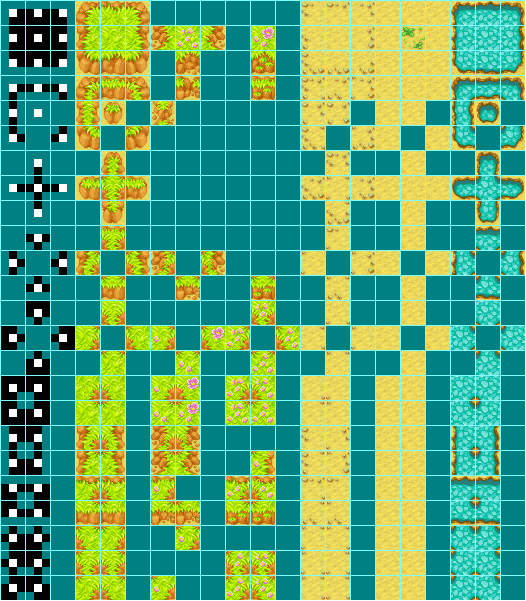
\includegraphics[width=0.8\textwidth]{tilemap.png}
    \end{center}
    \caption{Tileset utilisé pour construire un monde}
    \end{figure}

    \begin{figure}[ht]
    \begin{center}
        
\includegraphics[width=0.8\textwidth]{pokemonLatex.png}
    \end{center}
    \caption{Tileset utilisé pour les pokémons}
    \end{figure}



    \clearpage
    \section{Description et conception des états}

    \subsection{Description des états}
    Un état du jeu est formé d'une carte qui est statique au cours du temps et d'une liste de joueurs dont l'état varie au cours du jeu.

    \subsubsection{Etat de la carte}
    Une carte est composée de plusieurs couches, d'une longueur en nombre de tiles, d'une largeur en nombre de tiles, de la largeur de ses tiles en pixels, de la longueur de ses tiles en pixels et d'un tileset.

    Chaque couche de la carte comporte un nom, une largeur et une longueur en nombre de tiles, d'une position correspondant à la position de sa première tile et d'une liste d'index correspondant aux tiles utilisé pour chaque case, ces tiles doivent se trouver dans le tileset de la carte.

    Un tileset comprend une chaine de charactères correspondant au chemin de l'image du tileset et un identifiant.

    \subsubsection{Etat des joueurs}
    Un joueur est soit vivant, soit mort, soit un robot, soit un humain et il lui est attribué un pokemon en début de niveau/partie.

    Un pokemon possède une position, un nombre de point de vie à l'état t, un nom et un ensemble de statistiques qui lui sont attribués en début de partie.

    Ces statistiques correspondent aux attaques qu'il peut utiliser, à son nombre de point de vie en début de partie et son type (eau, feu, herbe).
    \subsection{Conception Logiciel}


    %\begin{landscape}
    %\begin{figure}[p]
    %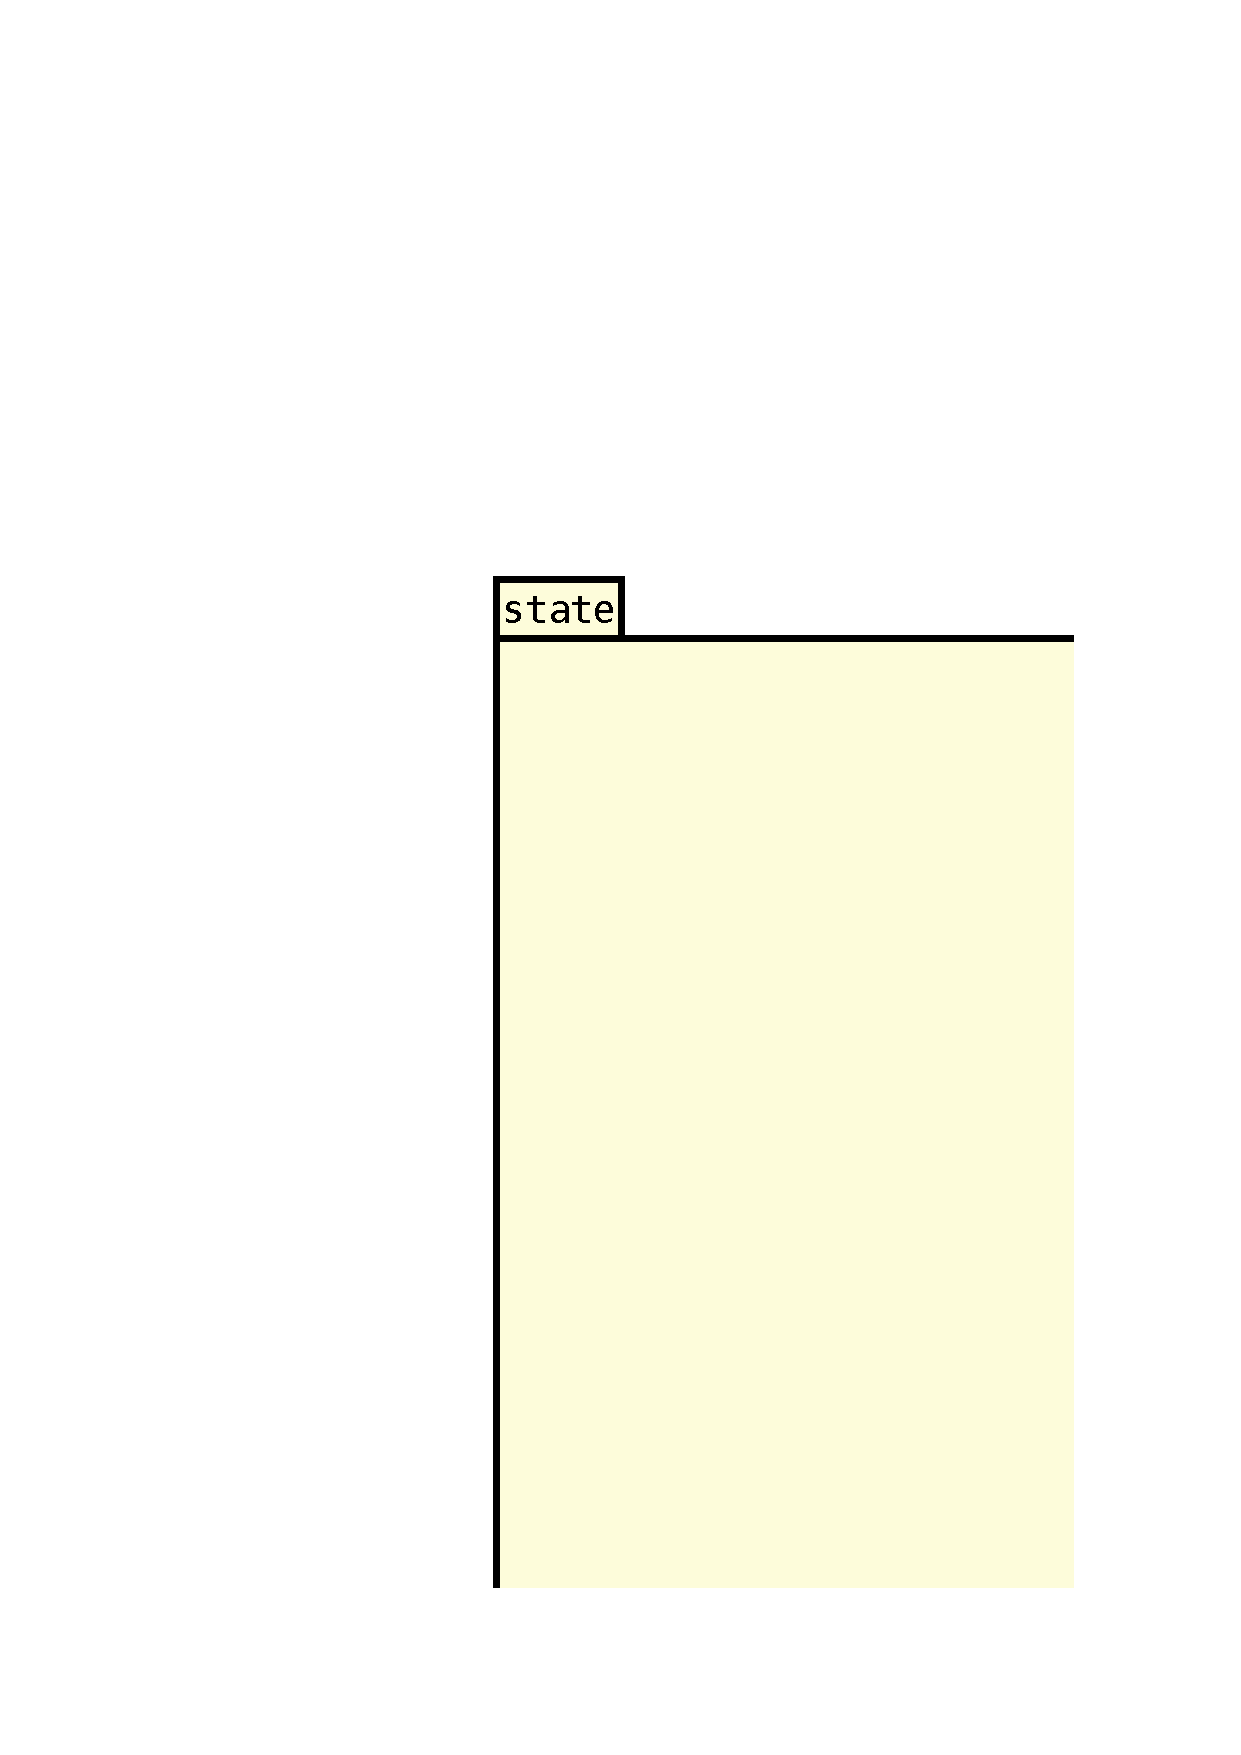
\includegraphics[width=0.9\paperheight]{state.pdf}
    %\caption{\label{uml:state}Diagramme des classes d'état.}
    %\end{figure}
    %\end{landscape}

    \clearpage
    \section{Rendu: Stratégie et Conception}

    \subsection{Stratégie de rendu d'un état}


    \subsection{Conception logiciel}

    %\begin{landscape}
    %\begin{figure}[p]
    %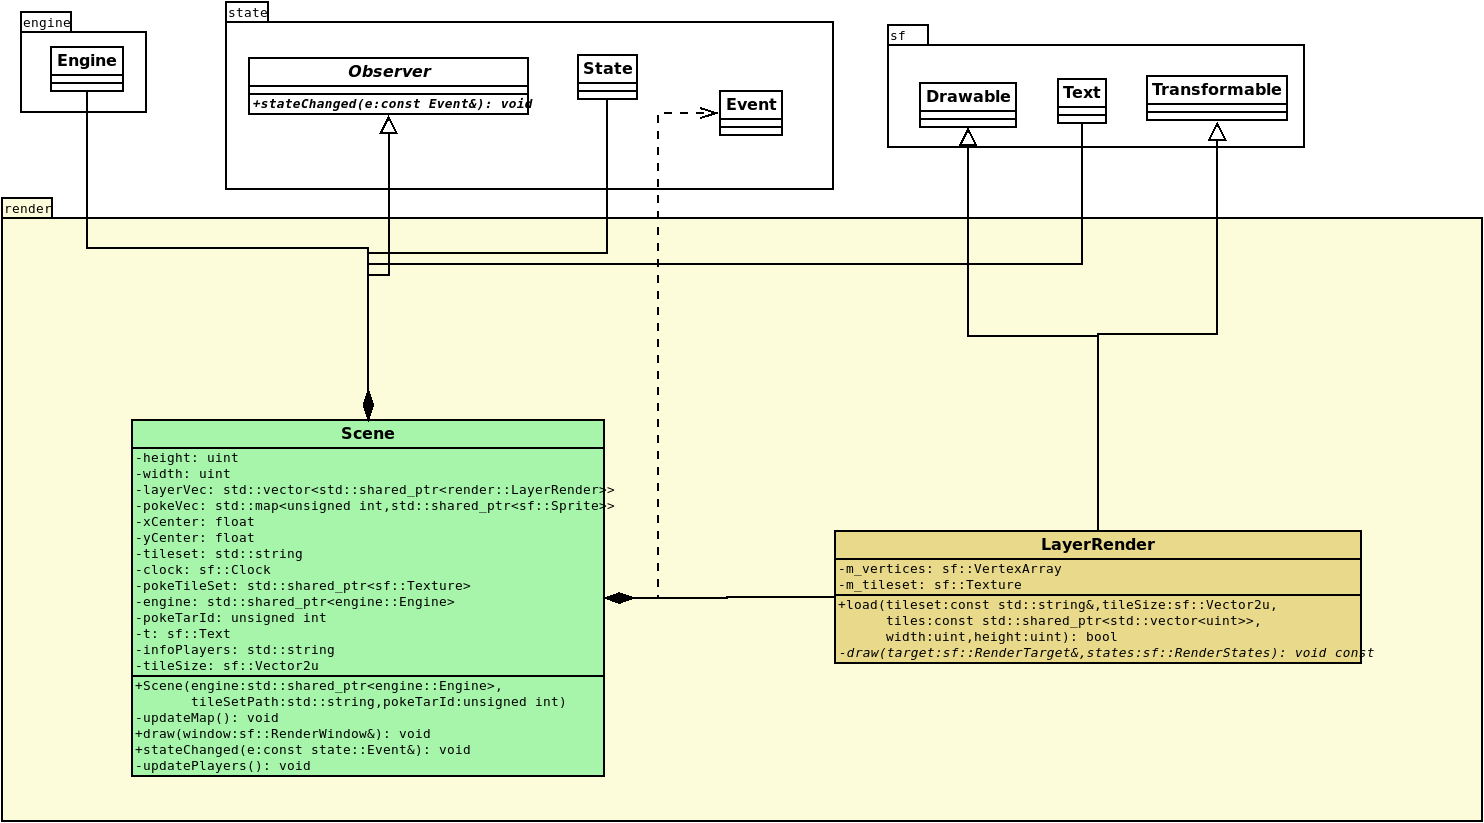
\includegraphics[width=0.9\paperheight]{render.pdf}
    %\caption{\label{uml:render}Diagramme des classes de rendu.}
    %\end{figure}
    %\end{landscape}

    \clearpage
    \section{Règles de changement d'états et moteur de jeu}

    \subsection{Règles}

    \clearpage
    \subsection{Conception logiciel}


    %\begin{landscape}
    %\begin{figure}[p]
    %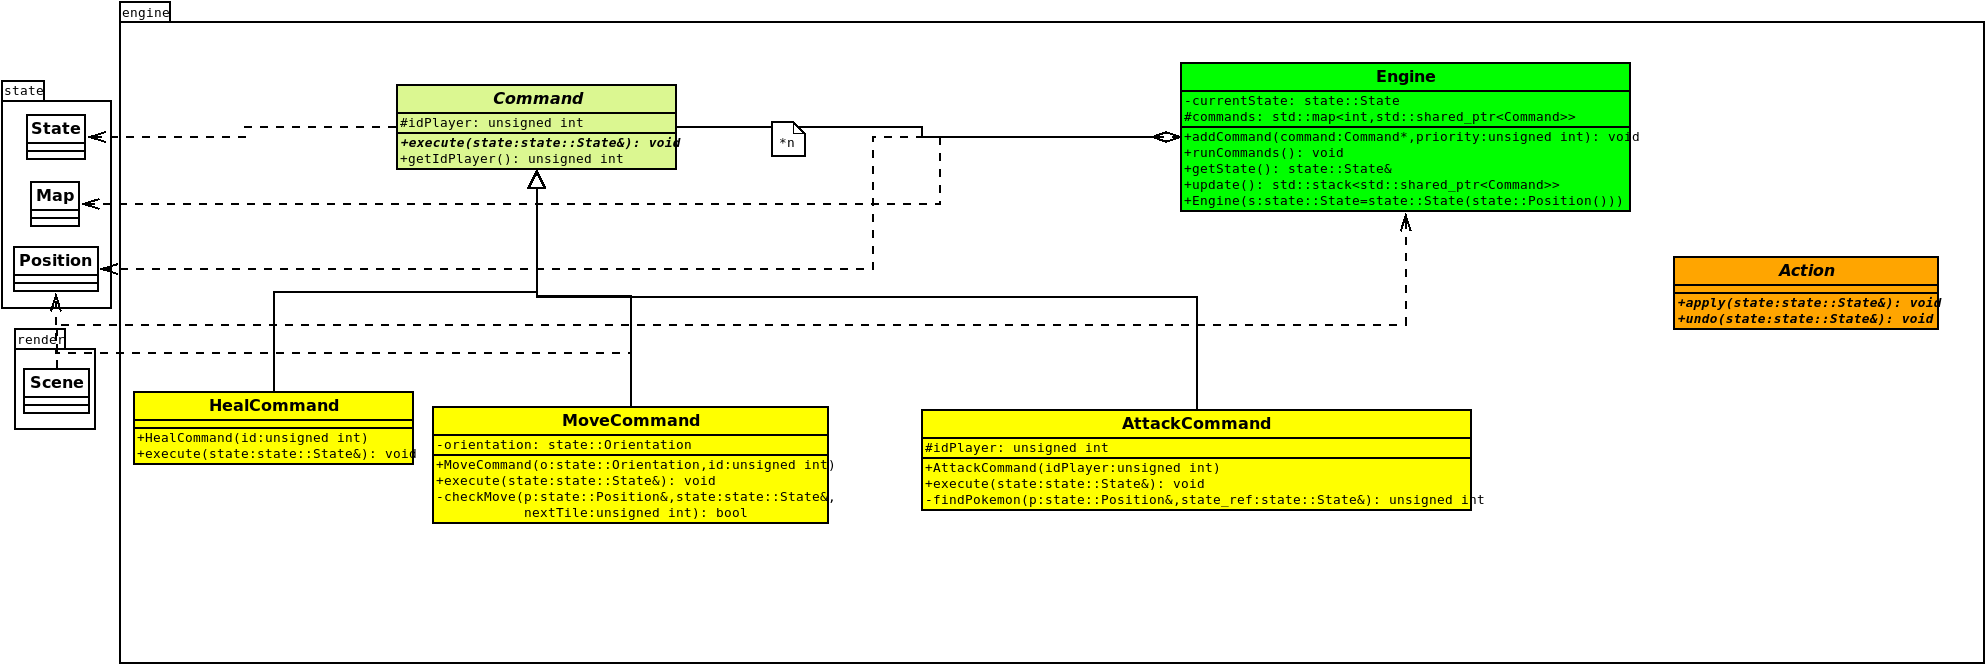
\includegraphics[width=0.9\paperheight]{engine.pdf}
    %\caption{\label{uml:engine}Diagramme des classes de moteur de jeu.}
    %\end{figure}
    %\end{landscape}


    \section{Intelligence Artificielle}

    \subsection{Stratégies}

    \clearpage
    \subsection{Conception logiciel}


    %\begin{landscape}
    %\begin{figure}[p]
    %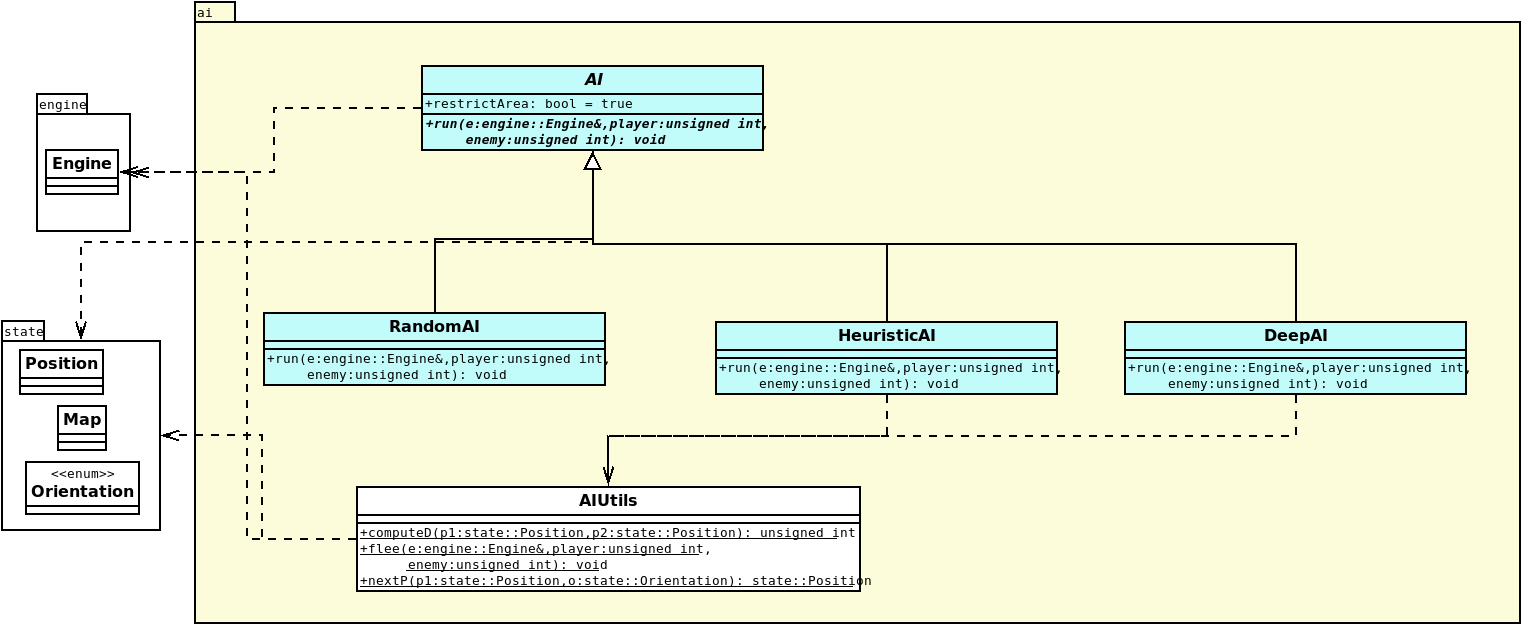
\includegraphics[width=0.9\paperheight]{ai.pdf}
    %\caption{\label{uml:ai}Diagramme des classes d'intelligence artificielle.}
    %\end{figure}
    %\end{landscape}


    \section{Modularisation}
    \label{sec:module}

    \subsection{Organisation des modules}

    \clearpage
    \subsection{Conception logiciel}


    %
    %\begin{landscape}
    %\begin{figure}[p]
    %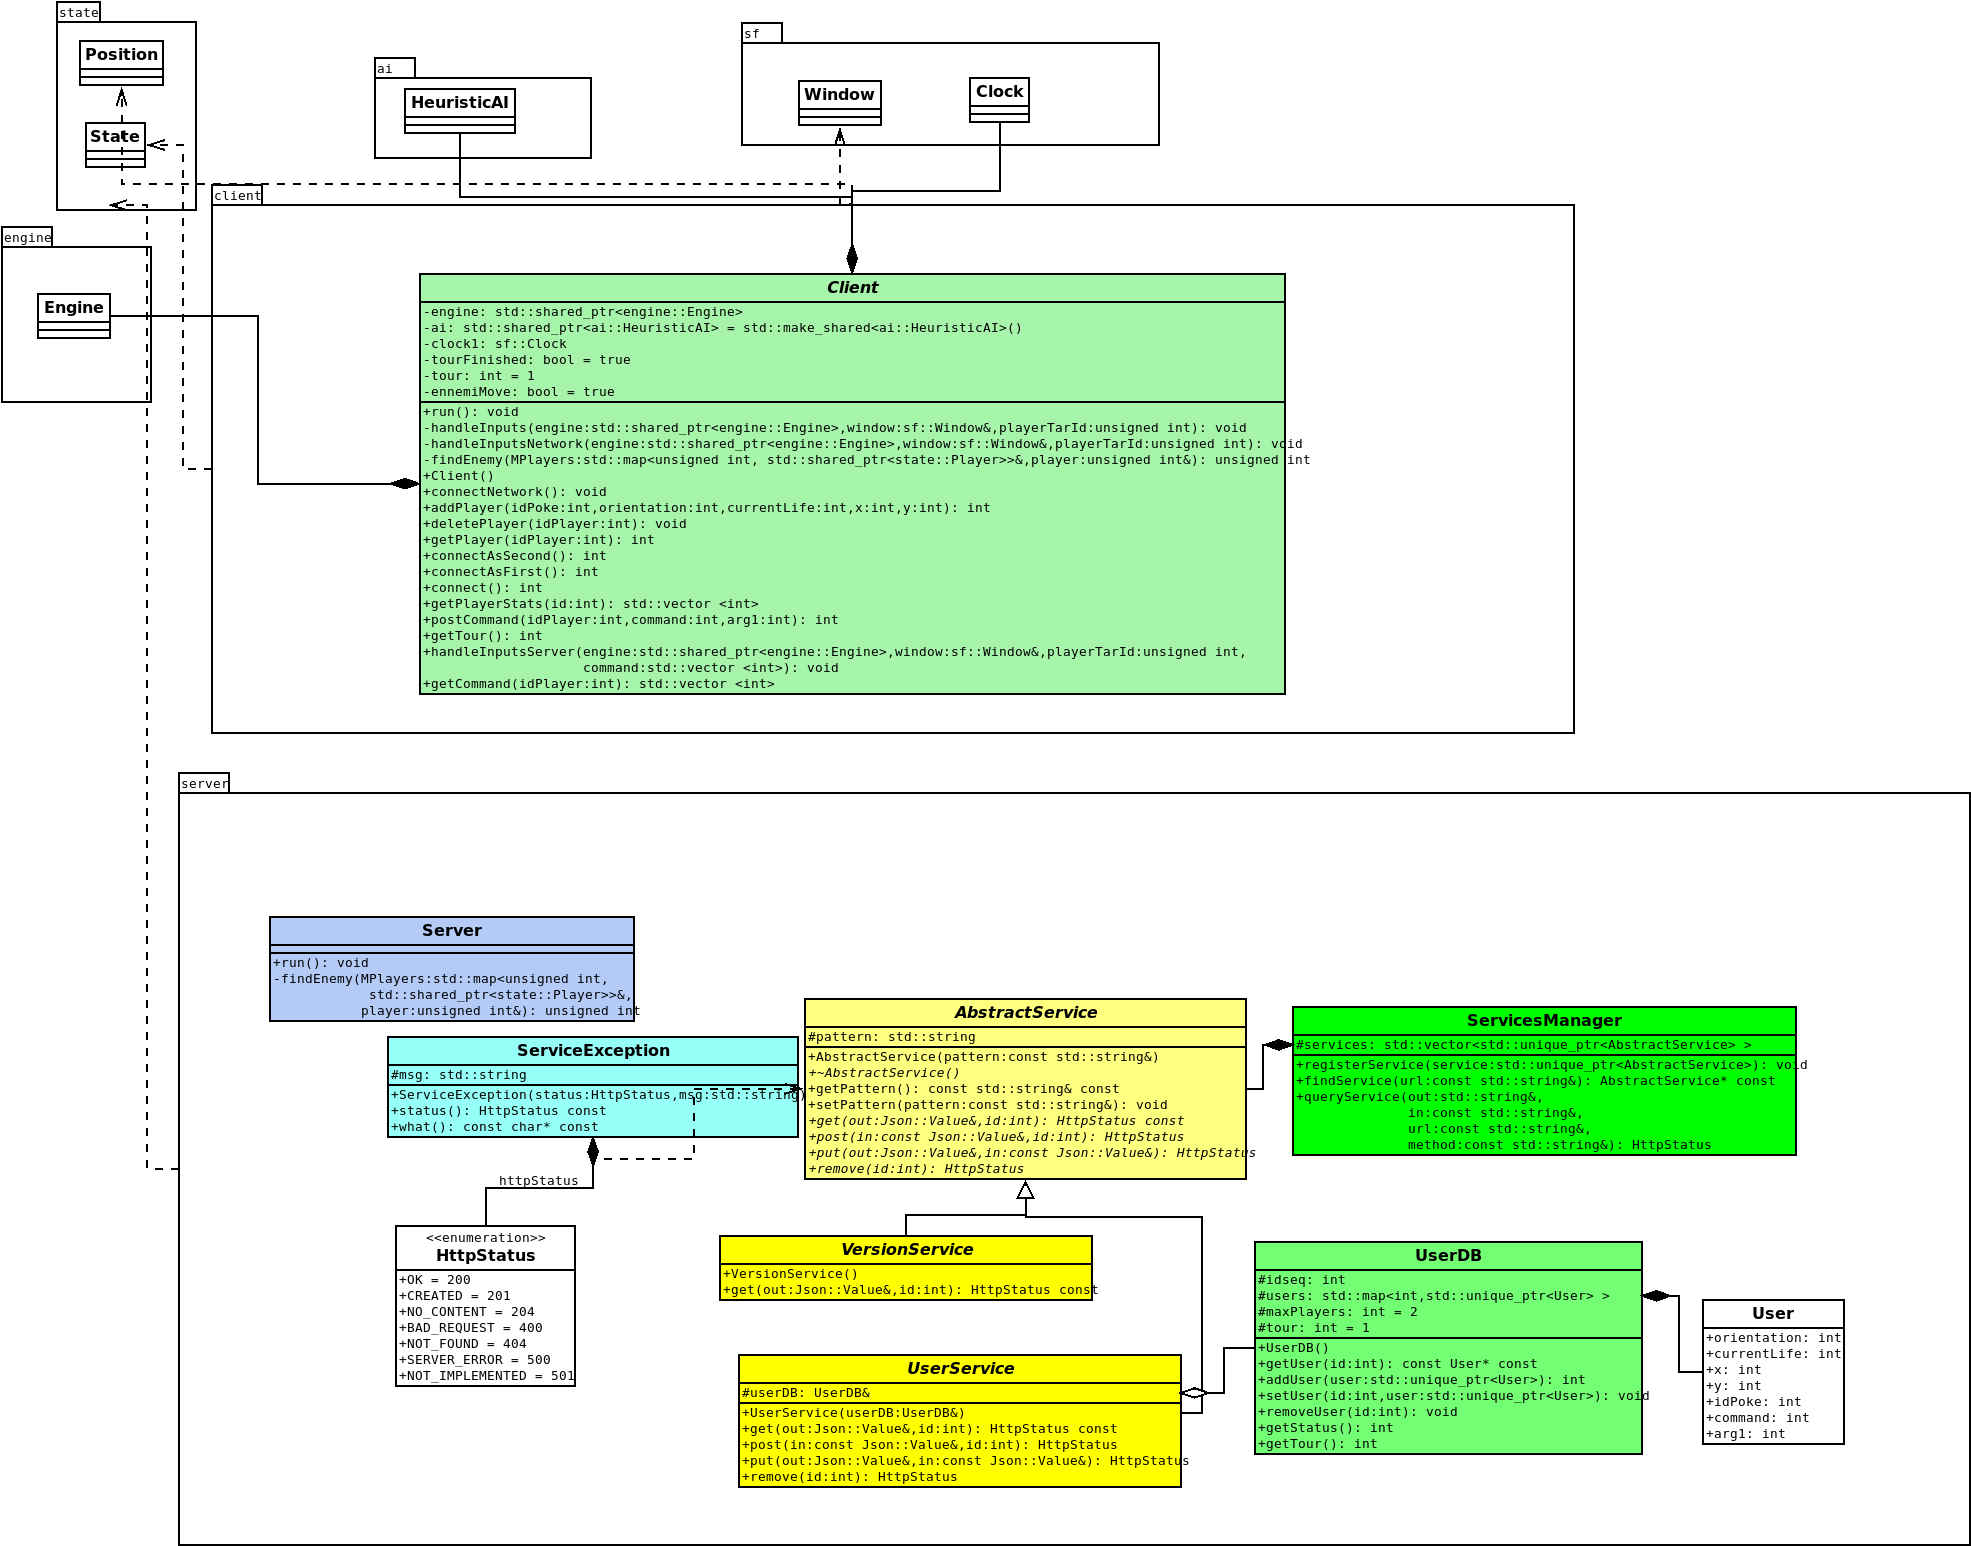
\includegraphics[width=0.9\paperheight]{module.pdf}
    %\caption{\label{uml:module}Diagramme des classes pour la modularisation.}
    %\end{figure}
    %\end{landscape}

\end{document}
